\chapter{User Interface}

To improve the quality, of one must build understandable and easy tasks as described in \textit{"Crowdsourcing, Collaboration and Creativity"} \cite{Kittur:2010}.

\section{Preliminary User Interface}\label{sec:FirstLayout}

For preliminary system tests, the system was first evaluated using a simple layout that only considers
\begin{itemize}
    \item The team
    \item The event
    \item The point in time
\end{itemize}

The first interface in Figure \ref{img:Layout1a} does not yet allow entering the positional information.

\begin{figure}[H]
    \centering
    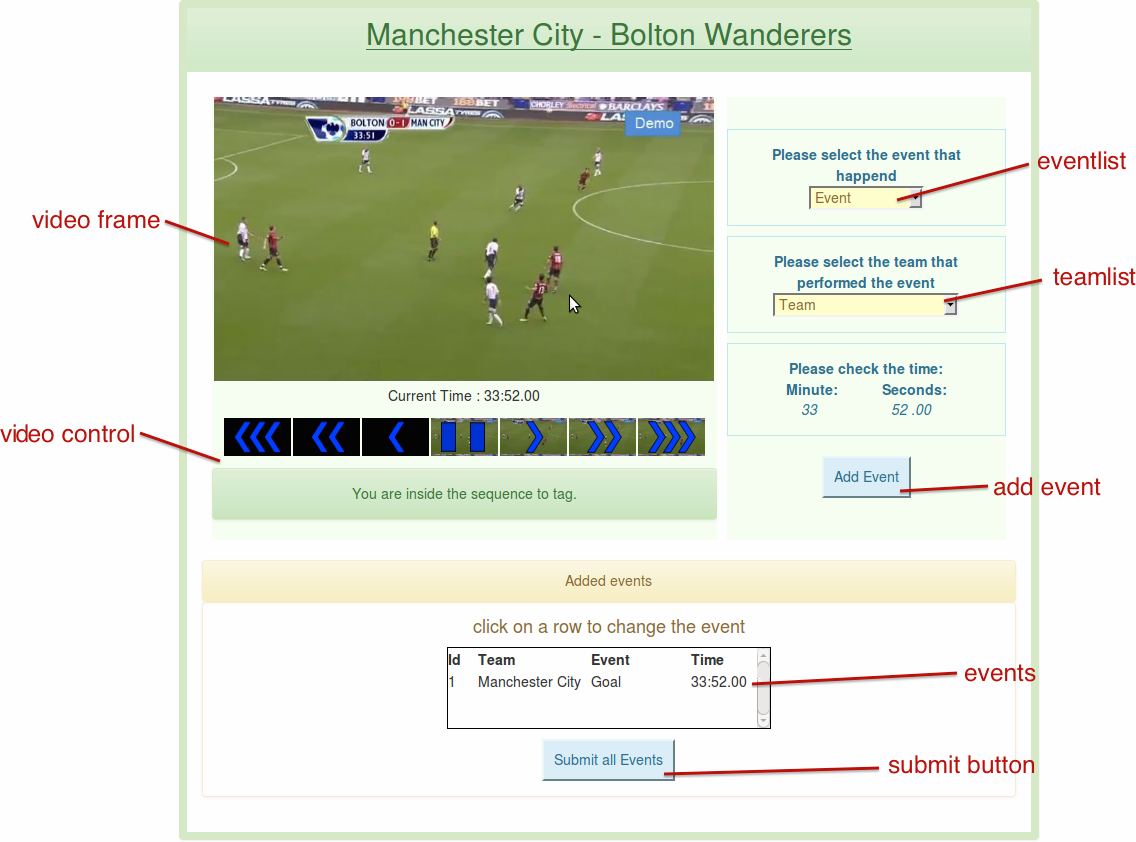
\includegraphics[width=0.78\textwidth]{layout/First}
    \caption{User interface that allows data entry}
    \label{img:Layout1a}
\end{figure}

To move through the video, workers have the possibility to use the keyboard, where a push on the spacebar plays and stops the video, and navigation can be done by using the left (backward) and right (forward) arrow keys to navigate through the movie.
Another possibility to change the position in the video file is to use the row under the video player. With this extension, the video can be controlled. By clicking on the images on the right side of the pause symbol \ref{img:pause} one can go forward. The number of arrows indicates how fast forward and backward a user goes by clicking, where every arrow is equated by a tenth second.


\begin{figure}[H]
    \centering
    
\includegraphics[scale=0.8]{layout/pause}
    \caption{Pause symbol used in the movie controller}
    \label{img:pause}
\end{figure}

The background of the navigation symbols shows the video frames at the corresponding time. Black background images indicate that the user is outside his task.

If the worker navigates the video file to a position where he sees an action he to chose the appropriate event from the drop-down list. The third item workers need to select is the team appertaining to the selected event. By clicking on the list, users will see both team names and the corresponding shirt color.
After selecting all items, clicking the "Add Event" button will submit the event to the list containing all entered events.
\newline
Those steps have to be repeated for the whole scene until all actions in the task's temporal sequence are added to the list.
By clicking on a row in the events list, the video will jump to the entered time and the drop-down lists will show the entered values. Workers now have the possibility to change any information of this data set or delete the event. If they do not want to do either of these two manipulations they can cancel the editing mode.

After finishing his task determined by the sequence end, the worker must click the submit button to enter the events in the database and receive his token.

The evaluation of this system by using Microworkers is made in Section \ref{sec:firstTest}.

\newpage

\section{Second Layout}\label{sec:SecondLayout}

Based on the results of the first test using the preliminary user interface, the layout was adjusted.

\begin{figure}[H]
    \centering
    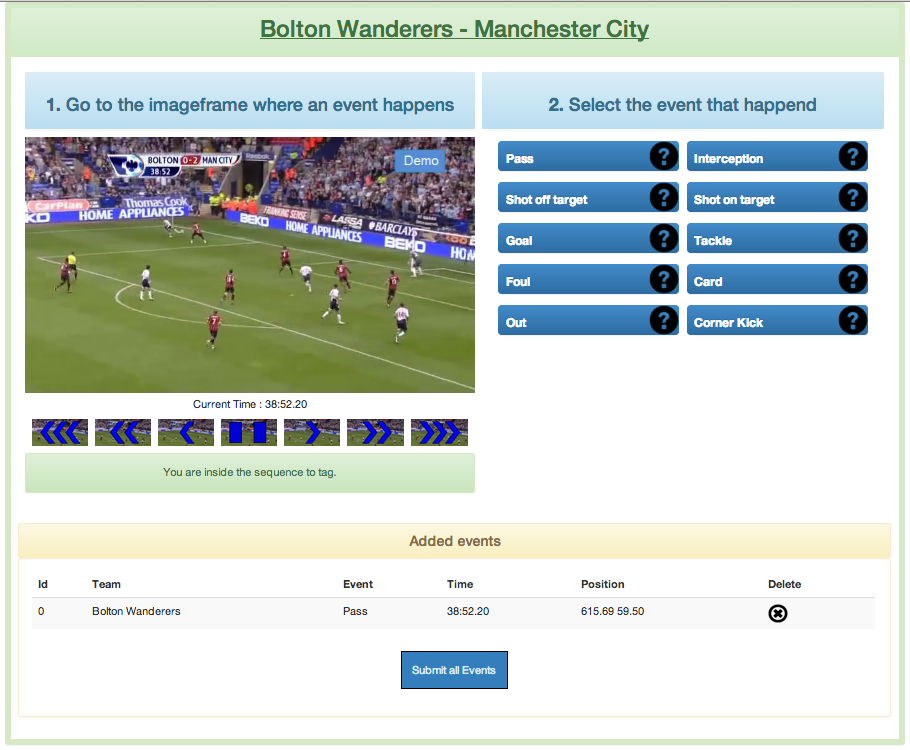
\includegraphics[width=0.8\textwidth]{layout/Second}
    \caption{Second layout at starting position of video snippet}
    \label{img:Layout2}
\end{figure}

To guide the user in the choices, some titles with numbers were added to all steps a user has to enter.
The input menu is split into different views, where the user first has to select the event by clicking the corresponding button. To help users select the right event, every event button contains a help text which shows up when hovering over the question mark in it.
After selecting the event the event view will be replaced by a similar view where the user have to select the appropriate team.
After selecting the team, the team frame also will be hidden and a new view will become visible. In this view, workers will see a soccer field where they have to enter the position where the event happens, by clicking on the appropriate position on the field.

After setting the position, participants must click on an "Add Event" button, similar the first layout, to enter the data. To encourage users to enter all events in the sequence and not stop after adding the first one, they will be asked to check the rest of the sequence for more events and to add them, because preliminary tests have shown that users often add just one event and then stop, rather than to check the sequence for more and to add them.

In addition, the possibility to edit an event was removed; instead, a delete row containing a delete icon was added to the events list, where users can delete a wrong event by selecting the appropriate icon in the table.

